\section{Resultados}
\label{sec:resultados}

\subsection{Selección de estudios}
\label{sec:res-seleccion}
% PRISMA ítems 16a (selección de estudios) y 16b (estudios excluidos)

% Generado por analysis/src/tablas/figuras_tex.py — no editar a mano.
\begin{figure*}[!tbp]
\centering
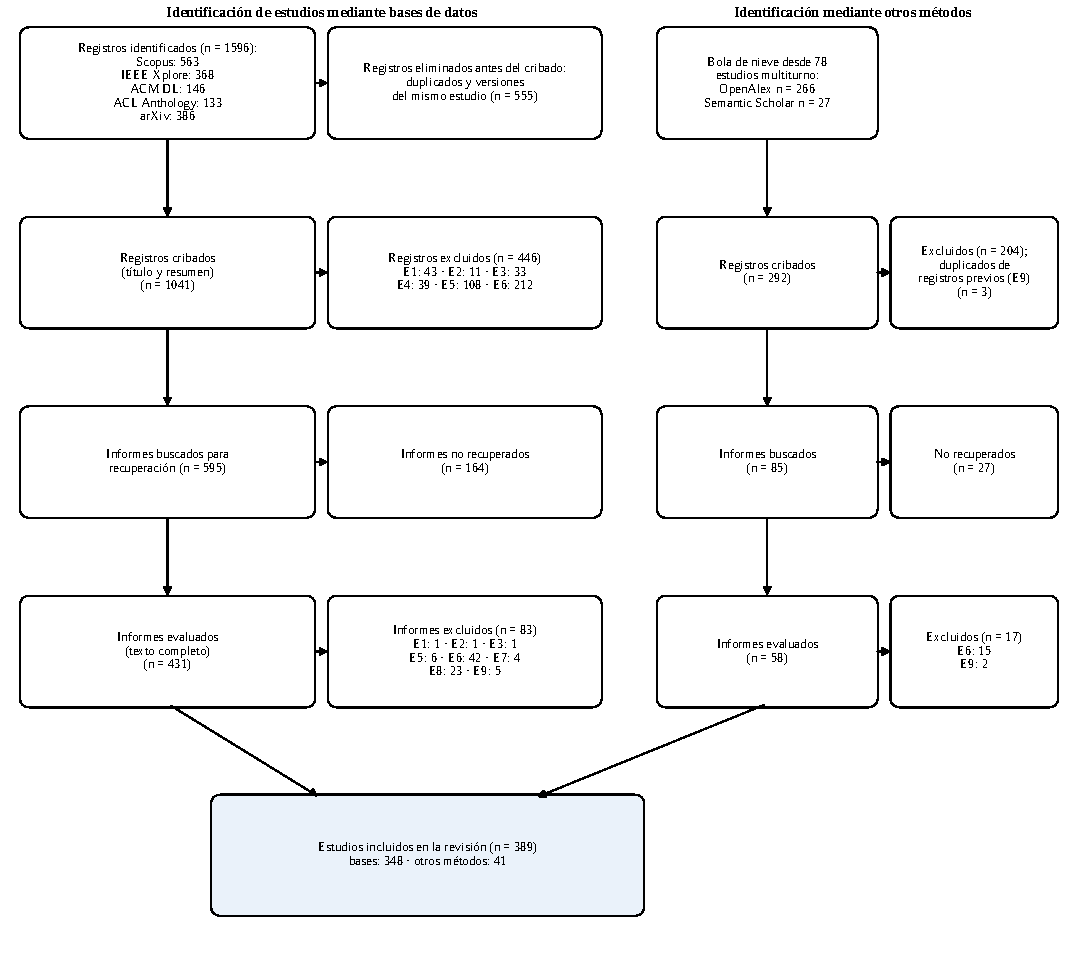
\includegraphics[width=7.12in,height=0.85\textheight,keepaspectratio]{prisma_flujo}
\caption{Diagrama de flujo PRISMA 2020 de la selección de estudios. E1–E9: códigos de exclusión del protocolo; E9 = informe secundario de un estudio ya incluido (versiones preprint/publicada o doble indexación), cuyo identificador se conserva en el informe primario.}
\label{fig:prisma_flujo}
\end{figure*}


La \cref{fig:prisma_flujo} presenta el flujo de la selección. En el brazo de bases de datos se identificaron \nIdentificados{} registros en las \nBases{} fuentes y se eliminaron \nDuplicados{} duplicados, de modo que se cribaron \nCribados{} títulos y resúmenes. El cribado excluyó \nExcluidosCribado{} registros y se buscaron \nBuscados{} informes, de los cuales \nNoRecuperados{} no pudieron recuperarse. Se evaluaron \nEvaluados{} informes a texto completo, se excluyeron \nExcluidosTexto{} y se incluyeron \nIncluidosBases{} estudios.

El brazo de otros métodos partió de \nBolaSemillas{} estudios semilla del Nivel 2 y aportó \nBolaCandOA{} registros de OpenAlex y \nBolaCandSS{} de Semantic Scholar. Tras eliminar 1 duplicado se cribaron 292 registros, de los que se excluyeron 204. Se buscaron 85 informes, 27 no se recuperaron, 58 se evaluaron a texto completo y 17 se excluyeron, con \nIncluidosBola{} estudios incluidos. El corpus final suma \nEstudios{} estudios, de los cuales \nMultiturno{} son multiturno y \nUnTurno{} son de un turno (las ejecuciones de extracción suman más por los estudios reclasificados; \cref{sec:met-extraccion}).
% fuente: prisma_conteos.json

Los motivos de exclusión se registraron por código. En el cribado de título y resumen del brazo de bases predominó E6 (\nExclTRBasesESeis{} de los \nExcluidosCribado{}; estudio de un turno sin la vinculación de esquemas o la autocorrección como contribución central), seguido de E5 (\nExclTRBasesECinco{}; no es Text-to-SQL sobre bases de datos relacionales) y E1 (\nExclTRBasesEUno{}; publicado antes de 2019). En texto completo predominaron E6 (\nExclTCBasesESeis{} informes) y E8 (\nExclTCBasesEOcho{}; estudio de un turno sin evaluación en un \en{benchmark} público), seguidos de E5 (\nExclTCBasesECinco{} informes), E7 (\nExclTCBasesESiete{}; sin evaluación empírica cuantitativa) y E9 (\nExclTCBasesENueve{}; informe secundario de un estudio ya incluido). En el brazo de otros métodos, E6 fue el motivo de \nExclTROtrosESeis{} exclusiones en el cribado y de \nExclTCOtrosESeis{} en texto completo. La lista de informes excluidos a texto completo, con su motivo, se incluye en el \cref{app:excluidos}.
% fuente: prisma_conteos.json

Los informes no recuperados fueron \nNoRecuperados{} en el brazo de bases y 27 en el de otros métodos. Se describen por escenario en la \cref{sec:res-caracteristicas}.
% fuente: prisma_conteos.json

\subsection{Características de los estudios}
\label{sec:res-caracteristicas}
% PRISMA ítems 17 (características de los estudios) y 20a (características por síntesis)

% Generado por analysis/src/tablas/figuras_tex.py — no editar a mano.
\begin{figure}[!tbp]
\centering
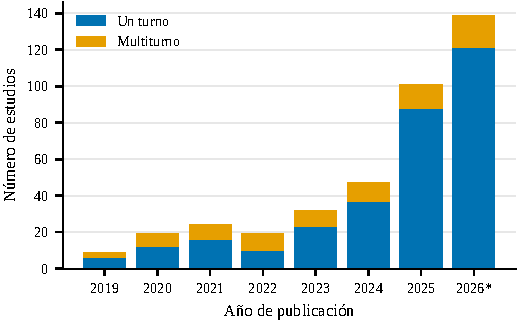
\includegraphics[width=\columnwidth,height=0.85\textheight,keepaspectratio]{pi0_anio_escenario}
\caption{Estudios incluidos por año de publicación y escenario (n = 390). *2026: año parcial (búsqueda del 11 de octubre de 2026).}
\label{fig:pi0_anio_escenario}
\end{figure}


La \cref{fig:pi0_anio_escenario} muestra los \nEstudios{} estudios por año de publicación y escenario. En 2019 se publicaron 9 estudios, 3 de ellos multiturno. En 2025 fueron 101, con 13 multiturno y 88 de un turno. En 2026, año parcial por la fecha de la búsqueda, se contabilizan 139 estudios: 18 multiturno y 121 de un turno.
% fuente: PI0.md, pi0_anio_escenario.csv

Por tipo de publicación, \nForoPreprint{} estudios son \en{preprints}, \nForoCongresoAestrella{} son congresos con clasificación CORE A* y \nForoRevistaQUno{} son artículos de revista del primer cuartil. El resto son congresos con clasificación CORE A (\nForoCongresoA{}), B (\nForoCongresoB{}) y C (\nForoCongresoC{}) o sin clasificación (\nForoCongresoSinRanking{}); artículos de revista de los cuartiles Q2 (\nForoRevistaQDos{}), Q3 (\nForoRevistaQTres{}) y Q4 (\nForoRevistaQCuatro{}) o sin cuartil (\nForoRevistaSinRanking{}); talleres (\nForoTallerSinRanking{}); y \nForoDesconocido{} con foro desconocido. El foro más frecuente es arXiv (\nVenueUno{} estudios), seguido de \en{Annual Meeting of the Association for Computational Linguistics} (\nVenueDos{}), \en{Findings of the ACL: ACL 2026} (\nVenueTres{}) y \en{Proceedings of the ACM on Management of Data} (\nVenueCuatro{}).
% fuente: PI0.md, pi0_foros.csv, pi0_venues_top.csv

El paradigma técnico principal por año se detalla en la \cref{fig:pi0_paradigma_anio} (\cref{app:figuras}). Hasta 2022 predominan el ajuste fino de modelos de lenguaje preentrenados y los modelos neuronales anteriores a ellos; el primer estudio con \en{prompting} de modelos de lenguaje grandes data de 2022. En 2026 el \en{prompting} reúne 54 estudios, los agentes 43 y el ajuste fino de modelos de lenguaje grandes 25. El ajuste fino de modelos preentrenados alcanza 19 estudios en 2023 y 3 en 2025.
% fuente: PI0.md, pi0_paradigma_anio.csv

Los pilares centrales difieren por escenario. Entre los estudios multiturno, \nPilarUnoMT{} tienen PI1 como contribución central y \nPilarDosMT{} tienen PI2; ningún estudio de un turno cumple esos dos pilares. PI3 es central en \nPilarTresMT{} estudios multiturno y \nPilarTresUT{} de un turno, y PI4 en \nPilarCuatroMT{} multiturno y \nPilarCuatroUT{} de un turno. Entre los estudios con PI3 central, 34 de 60 en 2026 no requieren entrenamiento (15 de 43 en 2025); para PI4 son 44 de 81 en 2026 (20 de 50 en 2025).
% fuente: PI0.md, pi0_pilares_escenario.csv, pi0_training_free.csv

Los informes no recuperados, que corresponden a ambos brazos de búsqueda, se distribuyen en 148 con señal de un turno y 43 con señal multiturno; la señal se asignó por la presencia de palabras clave de multiturno en el título o el resumen (\cref{sec:met-busqueda}).
% fuente: PI0.md, pi0_no_recuperados_escenario.csv, pi0_resultados.json

\subsection{Indicador D4}
\label{sec:res-d4}
% PRISMA ítems 20b (resultados de las síntesis) y 20d (sensibilidad)

El indicador D4 estricto es \DcuatroK{} de \DcuatroN{} estudios, es decir, \DcuatroPct~\% (IC 95~\% de Wilson, \DcuatroICinf{}--\DcuatroICsup{}~\%). El denominador son los estudios con PI3 o PI4 como contribución central, no los \nEstudios{} incluidos, porque esa es la población que define el indicador. Se trata de una proporción descriptiva dentro del marco de elegibilidad. El límite superior del intervalo es inferior al \umbralMayoria~\%, de modo que los estudios multiturno son una minoría de esta población. La versión laxa es de \DcuatroLaxoK{} de \DcuatroLaxoN{} estudios, \DcuatroLaxoPct~\% (IC 95~\% de \DcuatroLaxoICinf{} a \DcuatroLaxoICsup~\%), con la misma conclusión. En el Nivel 1, el acuerdo entre revisores en el campo que define D4 (pilares PI3/PI4 centrales) fue de $\kappa$ = \kappaCentral{} (PABAK \pabakCentral{}; $n$ = \nKappaCentral{}). El intervalo de Wilson cubre solo el error muestral y no esta incertidumbre de clasificación.
% fuente: PI0.md, pi0_resultados.json, revision_4f.json (A6_acuerdo_central_nivel1)

Como complemento \en{post hoc}, la proporción inversa mide qué parte de los estudios multiturno tiene la vinculación de esquemas o la autocorrección como contribución central: \DcompK{} de \DcompN{}, es decir, \DcompPct~\% (IC 95~\% de Wilson, \DcompICinf{}--\DcompICsup{}~\%). El intervalo contiene el \umbralMayoria~\%, de modo que no puede afirmarse que estos pilares sean mayoritarios ni minoritarios dentro de la investigación multiturno. De los demás estudios multiturno, \DcompRestoPIdos{} se centran en la restauración del contexto o la representación del estado (PI1 o PI2) y en \DcompRestoSinPilar{} no se registró un pilar central. Ambas proporciones comparten el numerador y responden a preguntas distintas: D4 describe el peso del escenario multiturno dentro de estos pilares, y el complemento, el peso de estos pilares dentro del escenario multiturno.
% fuente: pi0_resultados.json (D4.complemento_multiturno)

% Generado por analysis/src/tablas/figuras_tex.py — no editar a mano.
\begin{figure}[!tbp]
\centering
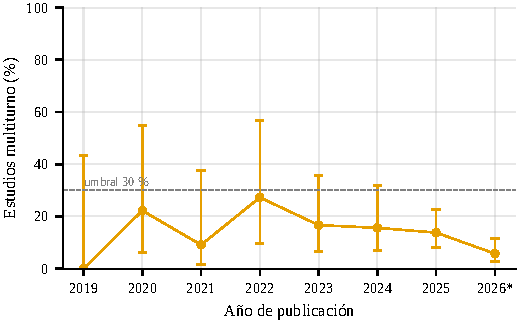
\includegraphics[width=\columnwidth,height=0.85\textheight,keepaspectratio]{d4_tendencia}
\caption{Indicador D4 por año: proporción de estudios multiturno entre los estudios con vinculación de esquemas o autocorrección (PI3/PI4) como contribución central, con IC 95 \% de Wilson. Línea discontinua: umbral pre-especificado del 30 \%. *2026: año parcial, excluido de la prueba de tendencia.}
\label{fig:d4_tendencia}
\end{figure}


La \cref{fig:d4_tendencia} muestra la proporción anual. La prueba de Cochran--Armitage para 2019--2025 no detecta tendencia (estadístico de $-0{,}6$; $p$ exacta bilateral \DcuatroTendenciaP{}, con 10\,000 réplicas). Las proporciones anuales van de 0 de 5 estudios en 2019 a 12 de 87 en 2025 (13,8~\%), con intervalos anuales amplios en los primeros años. El año 2026, parcial y fuera de la prueba principal, registra 7 de 122 estudios (5,7~\%; IC 95~\% de 2,8 a 11,4~\%). Como sensibilidad, la prueba que incluye 2026 da $p$ = \tendenciaConP{} (dirección decreciente, no significativa al 0,05); la prueba registrada se mantiene como principal.
% fuente: PI0.md, pi0_resultados.json, d4_tendencia.csv, revision_4f.json (A3_tendencia_2019_2026)

% Generado por analysis/src/tablas/tablas.py — no editar a mano.
\begin{table}[!tbp]
\centering
\caption{Indicador D4 (proporción multiturno) y análisis de sensibilidad, con IC de Wilson al 95 \%. Conclusión de la regla pre-especificada en todas las variantes: «considerablemente menos investigado». Tendencia 2019--2025 (Cochran--Armitage, \num{10000} réplicas): $p$ = \num{0.95}; 2026 (año parcial) se informa aparte: 7/122.}
\label{tab:d4}
\footnotesize
\begin{tabular}{@{}l r r r c@{}}
\toprule
Análisis & $k$ & $n$ & D4 (\%) & IC 95 \% \\
\midrule
Principal (estricto) & 34 & 302 & \num{11.3} & \num{8.2}--\num{15.3} \\
Laxo & 49 & 317 & \num{15.5} & \num{11.9}--\num{19.9} \\
Sin \en{preprints} & 23 & 177 & \num{13.0} & \num{8.8}--\num{18.7} \\
Solo búsqueda en bases & 34 & 273 & \num{12.5} & \num{9.0}--\num{16.9} \\
Foros de primer nivel (A5) & 15 & 116 & \num{12.9} & \num{8.0}--\num{20.2} \\
Con no recuperados, cota (A4) & 77 & 493 & \num{15.6} & \num{12.7}--\num{19.1} \\
\bottomrule
\end{tabular}
\end{table}


La \cref{tab:d4} resume las sensibilidades. Las variantes sin \en{preprints}, solo con búsquedas en bases y solo con foros de primer nivel conservan la lectura de minoría. La cota extrema que incorpora los informes no recuperados, con el supuesto de que todos cuentan en el denominador y los de señal multiturno también en el numerador, da \DcuatroCotaK{} de \DcuatroCotaN{} estudios (\DcuatroCotaPct~\%) y un límite superior de \DcuatroCotaICsup~\%; el \DcuatroCotaK{} es el numerador de esa cota y no el total de estudios multiturno; también queda por debajo del \umbralMayoria~\%. La estimación probabilística, que aplica a los informes no recuperados las tasas observadas entre los recuperados, da D4 $\approx$ \DcuatroProbPct~\%. La regla de contingencia por volumen del Nivel 1 no se activó, porque el texto completo de un turno fue inferior a 400 informes.
% fuente: PI0.md, sensibilidad.json, revision_4f.json (A7_cota_probabilistica)

\subsection{Panorama bibliométrico exploratorio}
\label{sec:res-bibliometria}
% PRISMA ítem 17 (características de los estudios; análisis exploratorio, no preespecificado)

Este panorama bibliométrico es un análisis exploratorio y descriptivo (enmienda A6) que no modifica ninguna conclusión pre-especificada. OpenAlex resolvió \nResueltosOA{} de los \nEstudios{} estudios en la consulta del \fechaOpenalex{}; los \nNoResueltosOA{} restantes no cuentan con datos bibliométricos.
% fuente: bibliometria_resultados.json

% Generado por analysis/src/tablas/figuras_tex.py — no editar a mano.
\begin{figure*}[!tbp]
\centering
\begin{minipage}[b]{0.56\textwidth}\centering
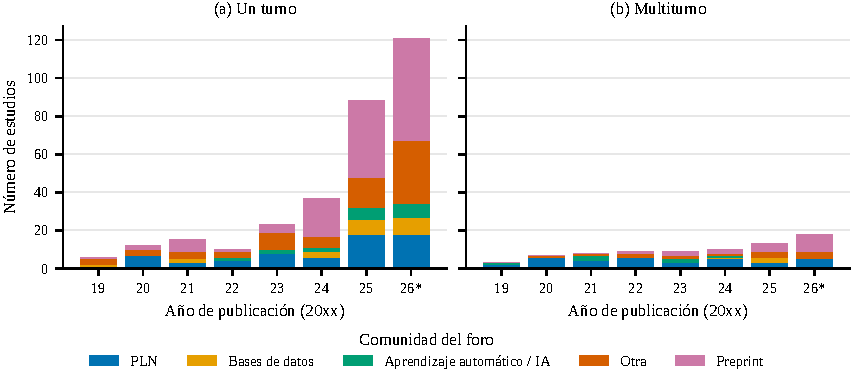
\includegraphics[width=\linewidth]{bib_comunidad}\\(a)\\[3pt]
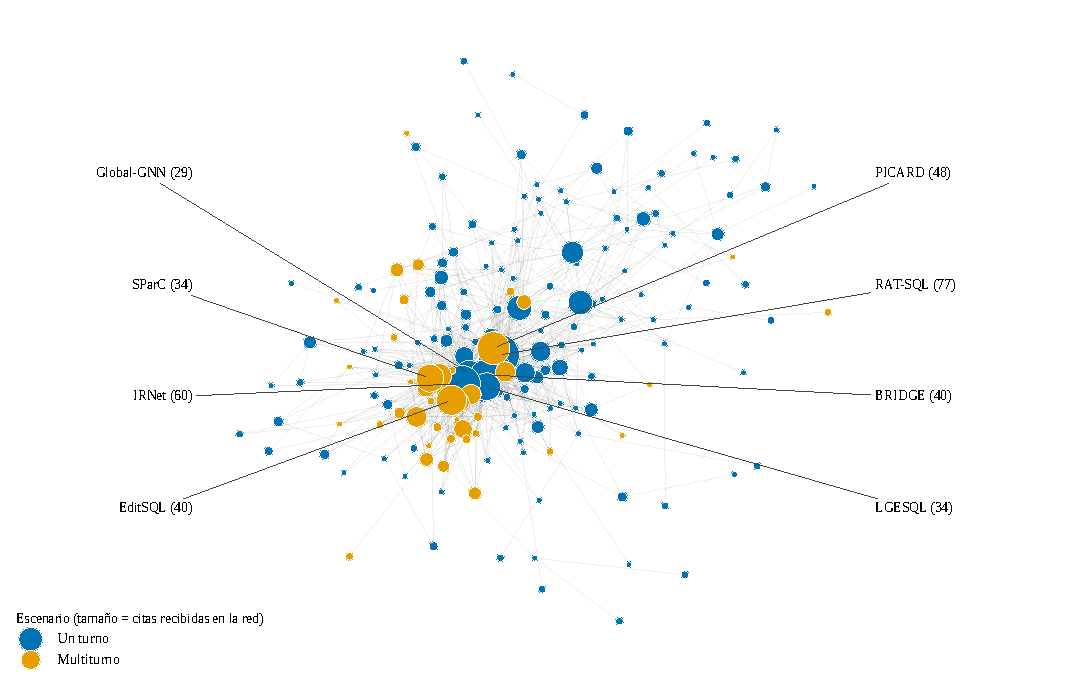
\includegraphics[width=\linewidth]{bib_red_citas}\\(b)
\end{minipage}\hfill
\begin{minipage}[b]{0.42\textwidth}\centering
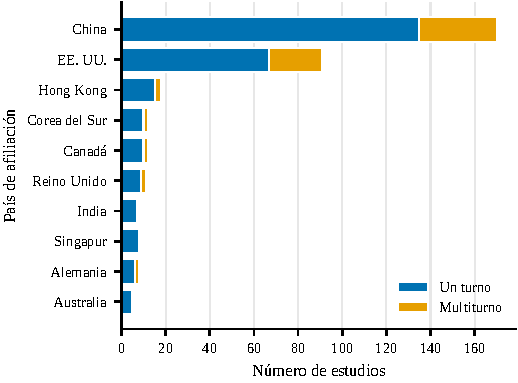
\includegraphics[width=0.82\linewidth]{bib_paises}\\(c)\\[3pt]
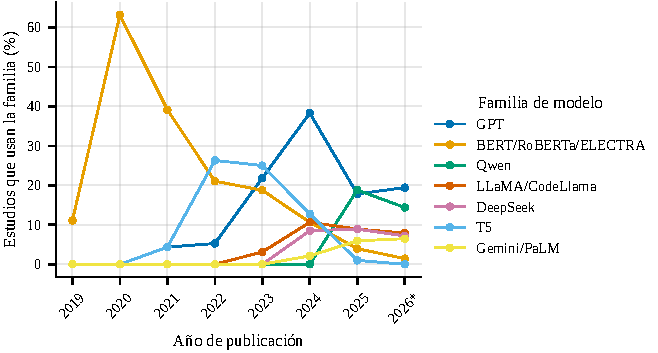
\includegraphics[width=\linewidth]{bib_modelos}\\(d)
\end{minipage}
\caption{Panorama bibliométrico exploratorio (enmienda A6). (a) Comunidad de investigación del foro de publicación, por año: (a) estudios de un turno; (b) estudios multiturno. *2026: año parcial. (b) Red de citas entre los estudios incluidos con al menos un vínculo (184 de 389 estudios; 841 citas; fuente: OpenAlex, 2026-10-13). Etiquetas: los ocho estudios más citados dentro de la red, con su número de citas. (c) Los diez países con más estudios incluidos, por escenario. Un estudio se cuenta en cada país con al menos un autor afiliado (fuente: OpenAlex, 2026-10-13). (d) Familias de modelos base por año (porcentaje de los estudios del año que mencionan la familia; un estudio puede usar varias). En el Nivel 1 solo se registraron los modelos citados en las páginas 1–2, por lo que el uso real está subestimado. *2026: año parcial.}
\label{fig:bib_panorama}
\end{figure*}


El panel~(a) de la \cref{fig:bib_panorama} clasifica el foro de publicación en cinco comunidades. Entre los estudios multiturno, \nComunidadPlnMT{} se publicaron en foros de procesamiento del lenguaje natural, \nComunidadBasesDatosMT{} en foros de bases de datos, \nComunidadAprendizajeMT{} en foros de aprendizaje automático o inteligencia artificial y \nComunidadOtraMT{} en otros foros, y \nComunidadPreprintMT{} son \en{preprints}. Entre los estudios de un turno, las cifras son \nComunidadPlnUT{}, \nComunidadBasesDatosUT{}, \nComunidadAprendizajeUT{}, \nComunidadOtraUT{} y \nComunidadPreprintUT{}, respectivamente.
% fuente: bib_comunidad.csv, PI0.md

La red de citas entre los estudios incluidos (panel~(b)) reúne \nCitasRed{} citas entre \nConVinculo{} estudios con al menos un vínculo, mientras que \nAislados{} estudios quedan aislados. Por dirección, hay \nCitasUTUT{} citas de un turno a un turno, \nCitasUTMT{} de un turno a multiturno, \nCitasMTMT{} de multiturno a multiturno y \nCitasMTUT{} de multiturno a un turno. La mediana de citas por año desde la publicación es de \citasMedMT{} en los estudios multiturno y de \citasMedUT{} en los de un turno. Por tipo de afiliación, \nAfilAcademia{} estudios son solo de academia, \nAfilMixta{} combinan academia e industria, \nAfilIndustria{} son solo de industria y \nAfilSinDatos{} carecen de datos.
% fuente: bibliometria_resultados.json, PI0.md, leyendas.json

Respecto de los países (panel~(c)), China registra 170 estudios (35 multiturno y 135 de un turno) y Estados Unidos 91 (24 y 67); siguen Hong Kong con 18, Corea del Sur con 12 y Canadá con 12. En cuanto a las familias de modelos base (panel~(d)), BERT, RoBERTa y ELECTRA y T5 son las más mencionadas hasta 2022; GPT lo es en 2024 y en 2026, y Qwen en 2025. Claude y Qwen aparecen desde 2025, y DeepSeek desde 2024. En el Nivel 1 solo se registraron los modelos citados en las páginas 1 y 2, de modo que el uso real de cada familia está subestimado, y las cifras por país y por comunidad dependen de la cobertura de OpenAlex y de la clasificación de los foros.
% fuente: bib_paises.csv, bib_modelos_anio.csv, PI0.md

Los análisis de productividad y red de coautoría, y de frecuencia de términos en títulos y resúmenes, se publican en el repositorio del proyecto.


\subsection{Calidad de los estudios}
\label{sec:res-calidad}
% PRISMA ítem 18 (riesgo de sesgo en los estudios)

Se evaluó la calidad de los \nMultiturno{} estudios del Nivel 2. De ellos, \nUmbral{} alcanzan el umbral de validez del \umbralValidez{}~\% y \nBajoUmbral{} quedan por debajo: \cite{Kochedykov2023Conversing,Joshi2020Natural,Lehmann2022Building,Parmar2026StocksTalk,ToctoInga2026CHIMLE}. La mediana de la puntuación de validez es \validezMediana{}~\% (rango intercuartílico de 60,0 a 80,0~\%; rango de 20,0 a 100,0~\%). Los porcentajes por ítem usan como denominador los \nMultiturno{} estudios evaluados, mientras que las taxonomías y los efectos usan los \nUmbral{} que alcanzan el umbral, porque la síntesis en profundidad se restringe a ellos. El umbral se registró y excluye pocos estudios, de modo que la lectura con todos los estudios es igualmente informativa; los estudios de un turno no se evaluaron, por lo que los contrastes con ellos carecen de evaluación de calidad.
% fuente: CALIDAD.md

El perfil completo por ítem y por estudio figura en el \cref{app:calidad}. Entre los ítems de validez, CQ6 (ablación o análisis de errores) es completo en 68 estudios (88,3~\%), mientras que CQ2 (reproducibilidad de la técnica) lo es en 14 (18,2~\%) y CQ5 (métricas e historial reportados) en 19 (24,7~\%). Entre los ítems de reporte, CQ1 es completo en los 77 estudios y CQ8 (código o datos disponibles) está ausente en 24 (31,2~\%).
% fuente: CALIDAD.md

\subsection{Efectos de los componentes}
\label{sec:res-efectos}
% PRISMA ítems 19 (resultados individuales), 20b, 20c (heterogeneidad) y 22 (certeza de la evidencia)

% Generado por analysis/src/tablas/tablas.py — no editar a mano.
\begin{table*}[!tbp]
\centering
\caption{Efecto de los componentes en contrastes dentro del estudio (diferencia en puntos porcentuales frente a la variante sin el componente), estudios del Nivel 2 que alcanzan el umbral de validez ($n = 72$). Est.: estudios; Contr.: contrastes; Med.: mediana; Val.: validez media de los estudios de la clase; \textsuperscript{c}Estudios con $|\Delta| < 0{,}5$~pp. \textsuperscript{d}Confianza registrada rebajada un nivel por sesgo de notificación. Conf.: confianza inspirada en GRADE-CERQual.}
\label{tab:efectos}
\footnotesize
\begin{tabularx}{\textwidth}{@{}l >{\raggedright\arraybackslash}X r r r r c r r r l l@{}}
\toprule
Pilar & Clase de componente & Est. & Contr. & Med. (pp) & Rango (pp) & Est. $+/-/0$ & Contr. $+$ (\%) & Nulos\textsuperscript{c} & Val. (\%) & Conf. & Conf. pen.\textsuperscript{d} \\
\midrule
PI1 & Concatenación / historial & 3 & 16 & \num{0.6} & \num{0.2} a \num{2.0} & 3/0/0 & \num{87.5} & 1 & \num{66.7} & moderada & baja \\
PI1 & Otros componentes del pilar & 17 & 119 & \num{2.4} & \num{-0.2} a \num{25.0} & 16/1/0 & \num{92.4} & 2 & \num{77.1} & alta & moderada \\
PI1 & Reescritura de la pregunta & 5 & 46 & \num{2.0} & \num{-4.8} a \num{19.2} & 4/1/0 & \num{73.9} & 0 & \num{76.0} & alta & moderada \\
\addlinespace
PI2 & Grafo / estado estructurado & 11 & 74 & \num{2.9} & \num{0.5} a \num{32.0} & 11/0/0 & \num{95.9} & 0 & \num{79.1} & alta & moderada \\
PI2 & Otros componentes del pilar & 22 & 124 & \num{2.9} & \num{-0.7} a \num{17.8} & 21/1/0 & \num{91.9} & 0 & \num{76.8} & alta & moderada \\
PI2 & SQL / resultados previos & 7 & 41 & \num{5.7} & \num{-0.1} a \num{10.5} & 6/1/0 & \num{90.2} & 1 & \num{81.4} & alta & moderada \\
\addlinespace
PI3 & Otros componentes del pilar & 15 & 143 & \num{2.1} & \num{-0.2} a \num{25.0} & 14/1/0 & \num{87.4} & 2 & \num{75.3} & alta & moderada \\
PI3 & Vinculación de esquemas & 19 & 92 & \num{2.2} & \num{0.3} a \num{33.2} & 19/0/0 & \num{81.5} & 2 & \num{76.3} & alta & moderada \\
\addlinespace
PI4 & Aclaración / interacción con el usuario & 3 & 7 & \num{8.9} & \num{-19.1} a \num{43.0} & 2/1/0 & \num{71.4} & 0 & \num{80.0} & moderada & baja \\
PI4 & Auto\-consistencia / selección de candidatos & 2 & 9 & \num{1.1} & \num{0.2} a \num{2.0} & 2/0/0 & \num{88.9} & 1 & \num{70.0} & moderada & baja \\
PI4 & Autocorrección / retroalimentación de ejecución & 11 & 141 & \num{1.5} & \num{0.0} a \num{13.8} & 11/0/0 & \num{93.6} & 3 & \num{72.7} & moderada & baja \\
PI4 & Otros componentes del pilar & 11 & 90 & \num{4.1} & \num{-2.3} a \num{13.8} & 10/1/0 & \num{86.7} & 2 & \num{77.3} & alta & moderada \\
\bottomrule
\end{tabularx}
\end{table*}


% Generado por analysis/src/tablas/figuras_tex.py — no editar a mano.
\begin{figure*}[!tbp]
\centering
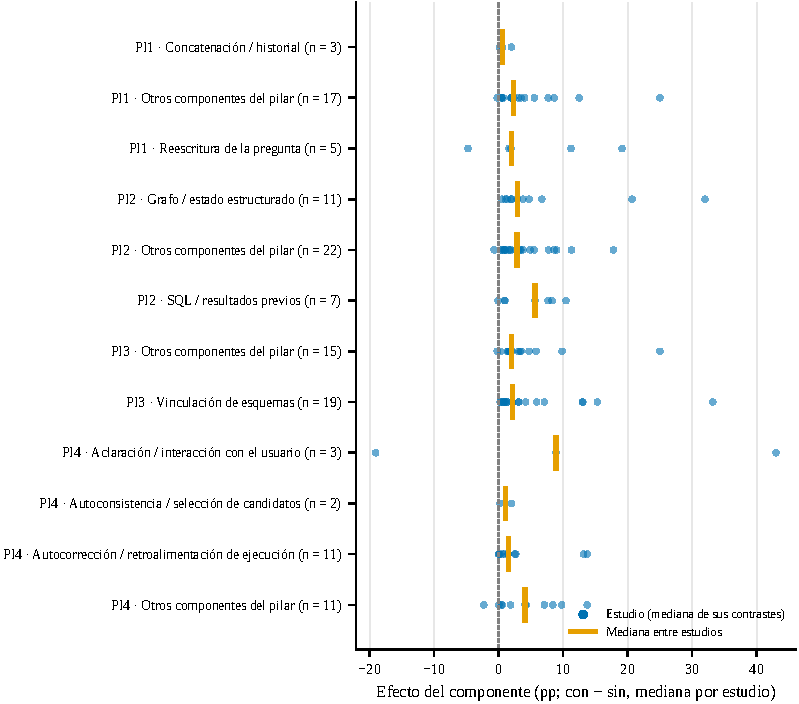
\includegraphics[width=5.33in,height=0.85\textheight,keepaspectratio]{pi_efectos_componentes}
\caption{Efecto de cada clase de componente según los contrastes dentro del estudio (activado frente a desactivado, mismo modelo base y configuración), en puntos porcentuales sobre métricas de exactitud. Cada punto es la mediana de los contrastes de un estudio; la barra, la mediana entre estudios. Síntesis sin metaanálisis (SWiM); estudios del Nivel 2 con validez $\geq$ 50 \%.}
\label{fig:pi_efectos_componentes}
\end{figure*}


La evidencia principal sobre el efecto de los componentes proviene de los contrastes dentro del estudio (componente activado frente a desactivado, con el mismo modelo base y configuración). Se analizaron los \nUmbral{} estudios del Nivel 2 que alcanzan el umbral de validez, agrupados por pilar y clase de componente (\cref{fig:pi_efectos_componentes} y \cref{tab:efectos}). Cada pilar incluye una clase «otros componentes», que reúne componentes heterogéneos.
% fuente: PI1.md, pi_efectos_componentes.csv

En PI1, la reescritura de la pregunta se evaluó en \efReescN{} estudios (\efReescPos{} con efecto positivo y \efReescNeg{} negativo) y la concatenación del historial en \efConcatN{} (\efConcatPos{} positivos), con medianas de \efReescMed{} y \efConcatMed{}~pp, respectivamente. Las dos clases provienen de contrastes distintos y no de una comparación directa dentro de un mismo estudio. En PI2, los \efGrafoN{} estudios sobre grafo o estado estructurado reportan efecto positivo, con mediana de \efGrafoMed{}~pp; de los \efSQLPrevN{} estudios sobre SQL o resultados previos, \efSQLPrevPos{} son positivos y \efSQLPrevNeg{} negativo, con mediana de \efSQLPrevMed{}~pp. En PI3, los \efVincN{} estudios sobre vinculación de esquemas son positivos, con mediana de \efVincMed{}~pp. En PI4, los \efAutocorrN{} estudios sobre autocorrección o retroalimentación de ejecución son positivos, con mediana de \efAutocorrMed{}~pp en \efAutocorrContr{} contrastes. La aclaración con el usuario tiene la mediana más alta de la \cref{tab:efectos} (\efAclarMed{}~pp) con solo \efAclarN{} estudios y \efAclarContr{} contrastes, y un rango de \efAclarMin{} a \efAclarMax{}~pp. La autoconsistencia se evaluó en \efAutoconsN{} estudios y \efAutoconsContr{} contrastes. Los componentes que la clasificación por nombre dejaba en «otros componentes» y que pertenecían a una clase existente se reasignaron a ella; el resto se desglosa en subclases en el \cref{app:otros}. Con un umbral de nulidad de $|\Delta| <$ \umbralNulo{}~pp, \nulosUmbral{} de los \nEstClase{} resultados estudio-clase son nulos (\cref{tab:efectos}).
% fuente: pi_efectos_componentes.csv, otros_subclases.csv, revision_4f.json (A4_nulos)

La confianza asignada a cada hallazgo es alta para la reescritura de la pregunta, el grafo o estado estructurado, el SQL o resultados previos y la vinculación de esquemas (\nConfAlta{} clases). Es moderada para la concatenación del historial (limitaciones metodológicas y suficiencia leves), la aclaración con el usuario (coherencia y suficiencia leves y pertinencia importante), la autoconsistencia (limitaciones metodológicas leves y suficiencia importante) y la autocorrección por ejecución (limitaciones metodológicas y pertinencia leves). Si se rebaja un nivel por sesgo de notificación, lectura añadida que no sustituye a la principal, las clases de confianza «alta» pasan a «moderada» y las de «moderada» a «baja». La clase «otros componentes», heterogénea, no recibe valoración de confianza. La \cref{tab:efectos} incluye la validez media de cada clase y ambas lecturas.
% fuente: confianza_hallazgos.csv, revision_4f.json (A4_confianza_penalizada)

En la sensibilidad, las medianas de la mayoría de las clases cambian poco al reincorporar los estudios bajo el umbral o al excluir los \en{preprints}. Al excluir los \en{preprints}, bajan las de SQL o resultados previos (de \efSQLPrevMed{} a \efSQLPrevMedSinPre{}~pp, \efSQLPrevNSinPre{} estudios) y vinculación de esquemas (de \efVincMed{} a \efVincMedSinPre{}~pp, \efVincNSinPre{} estudios). Al reincorporar los estudios bajo el umbral, la autocorrección por ejecución pasa de \efAutocorrN{} a \efAutocorrNTodos{} estudios (mediana de \efAutocorrMedTodos{}~pp) y «otros componentes» de PI3 sube de \efPItresOtrosMed{} a \efPItresOtrosMedTodos{}~pp.
% fuente: pi_efectos_componentes.csv, sensibilidad.json

La diferencia frente a la línea base propia es evidencia secundaria. Para el conjunto de pilares se registran 229 configuraciones de 43 estudios, con mediana de $\Delta$ de 2,8 pp; los archivos no la desagregan por pilar. Los valores individuales, cada uno en su \en{benchmark}, métrica e historial, se publican en el repositorio del proyecto y no se comparan entre estudios; el \cref{app:caracteristicas} recoge, cuando está disponible, el resultado principal de los estudios multiturno que alcanzan el umbral de validez.
% fuente: PI1.md, PI2.md, PI3.md, PI4.md

\subsection{PI1: restauración del contexto}
\label{sec:res-pi1}
% PRISMA ítems 19 (resultados individuales) y 20a (características por síntesis)

% Generado por analysis/src/tablas/tablas.py — no editar a mano.
\begin{table}[!tbp]
\centering
\caption{Taxonomía de PI1 y PI2: estudios del Nivel 2 que alcanzan el umbral de validez ($n = 72$). Un estudio puede tener varios códigos, por lo que los porcentajes de un campo pueden sumar más de 100.}
\label{tab:taxo-pi12}
\footnotesize
\begin{tabular}{@{}l r r@{}}
\toprule
Código & Estudios & \% \\
\midrule
\multicolumn{3}{@{}l}{\textit{PI1 · Técnica de restauración del contexto}} \\
\quad Concatenación del historial & 35 & \num{48.6} \\
\quad Reescritura de la pregunta & 12 & \num{16.7} \\
\quad Clasificación del discurso & 2 & \num{2.8} \\
\quad Resolución explícita de referencias & 2 & \num{2.8} \\
\quad No reportado & 25 & \num{34.7} \\
\multicolumn{3}{@{}l}{\textit{PI2 · Representación del estado}} \\
\quad Historial plano & 38 & \num{52.8} \\
\quad SQL previo (edición) & 11 & \num{15.3} \\
\quad Estructura explícita & 10 & \num{13.9} \\
\quad Grafo & 9 & \num{12.5} \\
\quad Memoria externa & 7 & \num{9.7} \\
\quad Ventana deslizante & 5 & \num{6.9} \\
\quad Resumen & 1 & \num{1.4} \\
\quad No reportado & 11 & \num{15.3} \\
\multicolumn{3}{@{}l}{\textit{PI2 · Actualización del estado}} \\
\quad Implícita (neuronal) & 34 & \num{47.2} \\
\quad Reglas deterministas & 16 & \num{22.2} \\
\quad Generativa (LLM) & 12 & \num{16.7} \\
\quad No reportado & 16 & \num{22.2} \\
\multicolumn{3}{@{}l}{\textit{PI2 · Coste del contexto}} \\
\quad Crece con los turnos & 36 & \num{50.0} \\
\quad Acotado & 14 & \num{19.4} \\
\quad No reportado & 22 & \num{30.6} \\
\bottomrule
\end{tabular}
\end{table}


La taxonomía de PI1 se basa en los \nUmbral{} estudios multiturno del Nivel 2 que alcanzan el umbral de validez (\cref{tab:taxo-pi12}). La técnica más frecuente es la concatenación del historial (35 estudios, 48,6~\%), seguida de la reescritura de la pregunta (12 estudios, 16,7~\%). La clasificación del discurso y la resolución explícita de referencias aparecen en 2 estudios cada una (2,8~\%), y 25 estudios (34,7~\%) figuran como «no reportado o no extraído», es decir, la técnica puede faltar en el informe o no haberse capturado en la extracción asistida por IA. Un estudio puede tener más de un código. Entre los insumos del historial, las preguntas previas están presentes en 59 estudios (81,9~\%), el SQL previo en 32 (44,4~\%), las respuestas del sistema en 13 (18,1~\%) y los resultados de ejecución en 3 (4,2~\%); 11 estudios (15,3~\%) no reportan el insumo.
% fuente: PI1.md

Entre los estudios que reescriben la pregunta figuran Rose-SQL~\cite{Zhou2026RoseSQL}, ACT-SQL~\cite{Zhang2023ACTSQL}, CQR-SQL~\cite{Xiao2022CQRSQL}, DIR~\cite{Li2023DIR}, QURG~\cite{Chai2023QURG} y FANDA~\cite{Liu2019FANDA}. CoE-SQL~\cite{Zhang2024CoESQL} y el trabajo de \en{self-play}~\cite{Liu2022Augmenting} concatenan el historial sin reescritura.

Respecto de la pregunta específica, los contrastes dentro del estudio se agrupan en clases distintas para la reescritura y para la concatenación, de modo que la comparación entre ambas es descriptiva y no procede de un mismo estudio. La mediana de la reescritura es de \efReescMed{}~pp (\efReescN{} estudios) y la de la concatenación de \efConcatMed{}~pp (\efConcatN{} estudios); en ambas clases la dirección es positiva en la mayoría de los estudios. El detalle, con la confianza de cada hallazgo, figura en la \cref{sec:res-efectos} (\cref{fig:pi_efectos_componentes} y \cref{tab:efectos}). Las diferencias frente a la línea base propia de los estudios con reescritura se reportan cada una en su \en{benchmark}, métrica e historial, y no se comparan entre sí; por ejemplo, ACT-SQL reporta +18,3~pp en CoSQL con la métrica QM y el historial SOLO\_PREGUNTAS.
% fuente: PI1.md

\subsection{PI2: representación y actualización del estado}
\label{sec:res-pi2}
% PRISMA ítems 19 (resultados individuales) y 20a (características por síntesis)

La base de PI2 son los mismos \nUmbral{} estudios del Nivel 2 (\cref{tab:taxo-pi12}). La representación más frecuente es el historial plano (38 estudios, 52,8~\%). Le siguen el SQL previo como base de edición (11 estudios, 15,3~\%), la estructura explícita (10, 13,9~\%), el grafo (9, 12,5~\%), la memoria externa (7, 9,7~\%), la ventana deslizante (5, 6,9~\%) y el resumen (1, 1,4~\%); 11 estudios (15,3~\%) no reportan la representación. La actualización del estado es implícita y neuronal en 34 estudios (47,2~\%), se basa en reglas deterministas en 16 (22,2~\%) y es generativa con un LLM en 12 (16,7~\%); otros 16 (22,2~\%) no la reportan.
% fuente: PI2.md

En cuanto al coste del contexto, 36 estudios (50,0~\%) crecen con el número de turnos, 14 (19,4~\%) lo acotan y 22 (30,6~\%) no lo reportan. Los trabajos con estructura explícita incluyen a Rose-SQL~\cite{Zhou2026RoseSQL}, el seguimiento de estados con aprendizaje en contexto~\cite{Hu2022InContext}, SemPlan~\cite{Teixeira2026SemPlan} y el modelado de estados de interacción~\cite{Wang2021Tracking}. Los de grafo son IGSQL~\cite{Cai2020IGSQL}, un grafo heterogéneo de interacción~\cite{Yu2021Interactionmodeling} y una red de relaciones híbrida dinámica~\cite{Hui2021Dynamic}. CoE-SQL~\cite{Zhang2024CoESQL} y EditSQL~\cite{Zhang2019EditSQL} editan el SQL previo.
% fuente: PI2.md

Los campos descriptivos del grafo no se reportan en 64 de los 72 estudios. Entre los 8 que sí los reportan, los nodos son elementos del esquema en 8 estudios, tokens de la pregunta en 4 y valores de la base de datos en 2, y el grafo es dinámico en 7 y estático en 1. Los archivos no incluyen el cruce entre tipo de representación y coste del contexto, solo las frecuencias marginales. Los contrastes dentro del estudio de las clases de grafo o estado estructurado (\efGrafoN{} estudios; mediana de \efGrafoMed{}~pp) y de SQL o resultados previos (\efSQLPrevN{} estudios; mediana de \efSQLPrevMed{}~pp) se presentan en la \cref{sec:res-efectos}.
% fuente: PI2.md

\subsection{PI3: vinculación de esquemas e inferencia de \en{joins}}
\label{sec:res-pi3}
% PRISMA ítems 19 (resultados individuales) y 20a (características por síntesis)

Entre los \nUmbral{} estudios del Nivel 2, la técnica de vinculación no se reporta en 22 (30,6~\%). Entre las reportadas predominan la coincidencia de cadenas (15 estudios, 20,8~\%), la ausencia de vinculación explícita (12, 16,7~\%) y el grafo del esquema (12, 16,7~\%); siguen el \en{prompting} de un LLM (10, 13,9~\%), el clasificador entrenado (9, 12,5~\%), la poda del esquema (7, 9,7~\%) y la recuperación por \en{embeddings} (6, 8,3~\%). La inferencia de \en{joins} es implícita en el modelo en 54 estudios (75,0~\%) y no se reporta en 16 (22,2~\%). Solo 2 estudios usan una inferencia no implícita: UniSAr~\cite{Dou2023UniSAr}, con caminos algorítmicos, y PG-GSQL~\cite{Wang2020PGGSQL}, con un grafo de claves foráneas y restricciones. Un total de 10 estudios (13,9~\%) reportan errores de \en{join}.
% fuente: PI3.md

% Generado por analysis/src/tablas/tablas.py — no editar a mano.
\begin{table}[!tbp]
\centering
\caption{Técnicas de PI3 y PI4 por escenario, con ambos brazos restringidos a los estudios cuya contribución central es PI3 o PI4 (misma regla de entrada): multiturno ($n = 34$) y un turno ($n = 268$). Un estudio puede tener varios códigos. Los estudios de un turno se extrajeron de las páginas iniciales (Nivel 1), por lo que la fila «no reportado» no es comparable entre escenarios. \textsuperscript{b}Técnica de un turno no trasladada al multiturno.}
\label{tab:contraste-pi34}
\footnotesize
\setlength{\tabcolsep}{4pt}
\begin{tabular}{@{}l r r@{}}
\toprule
Código & Multiturno & Un turno \\
\midrule
\multicolumn{3}{@{}l}{\textit{PI3 · Vinculación de esquemas}} \\
\quad LLM con \en{prompting} & 9 (\num{26.5}) & 68 (\num{25.4}) \\
\quad Poda del esquema & 7 (\num{20.6}) & 50 (\num{18.7}) \\
\quad Recuperación por \en{embeddings} & 5 (\num{14.7}) & 44 (\num{16.4}) \\
\quad Clasificador entrenado & 6 (\num{17.6}) & 41 (\num{15.3}) \\
\quad Ninguna explícita & 5 (\num{14.7}) & 31 (\num{11.6}) \\
\quad Grafo del esquema & 5 (\num{14.7}) & 27 (\num{10.1}) \\
\quad Coincidencia de cadenas & 8 (\num{23.5}) & 15 (\num{5.6}) \\
\quad No reportado & 8 (\num{23.5}) & 75 (\num{28.0}) \\
\multicolumn{3}{@{}l}{\textit{PI3 · Inferencia de \en{joins}}} \\
\quad Implícita en el modelo & 26 (\num{76.5}) & 55 (\num{20.5}) \\
\quad Grafo de claves foráneas & 1 (\num{2.9}) & 12 (\num{4.5}) \\
\quad Algorítmica (caminos) & 1 (\num{2.9}) & 8 (\num{3.0}) \\
\quad No reportado & 6 (\num{17.6}) & 193 (\num{72.0}) \\
\multicolumn{3}{@{}l}{\textit{PI4 · Mecanismo}} \\
\quad Retroalimentación de ejecución & 8 (\num{23.5}) & 90 (\num{33.6}) \\
\quad Verificador o crítico & 1 (\num{2.9}) & 58 (\num{21.6}) \\
\quad Autodepuración con LLM & 4 (\num{11.8}) & 40 (\num{14.9}) \\
\quad Autoconsistencia (votación)\textsuperscript{b} & 0 (\num{0.0}) & 36 (\num{13.4}) \\
\quad Aclaración con el usuario & 16 (\num{47.1}) & 6 (\num{2.2}) \\
\quad Abstención & 3 (\num{8.8}) & 8 (\num{3.0}) \\
\quad Reparación simbólica\textsuperscript{b} & 0 (\num{0.0}) & 6 (\num{2.2}) \\
\quad No reportado & 12 (\num{35.3}) & 105 (\num{39.2}) \\
\multicolumn{3}{@{}l}{\textit{PI4 · Señal}} \\
\quad Resultado de la ejecución & 7 (\num{20.6}) & 91 (\num{34.0}) \\
\quad Error del SGBD & 7 (\num{20.6}) & 56 (\num{20.9}) \\
\quad Juicio de un LLM & 3 (\num{8.8}) & 48 (\num{17.9}) \\
\quad Usuario & 15 (\num{44.1}) & 8 (\num{3.0}) \\
\quad Resultado vacío & 1 (\num{2.9}) & 7 (\num{2.6}) \\
\quad No reportado & 11 (\num{32.4}) & 120 (\num{44.8}) \\
\bottomrule
\end{tabular}
\end{table}


La \cref{tab:contraste-pi34} contrasta las frecuencias de cada código entre los \nCentralMT{} estudios multiturno y los \nCentralUT{} de un turno cuya contribución central es PI3 o PI4, con la misma regla de entrada en ambos brazos y sin aplicar el umbral de validez; por ello los recuentos multiturno difieren de los de la taxonomía anterior (p.\,ej., \nctLinkLlmPromptingMT{} frente a 10 estudios con \en{prompting} de un LLM). Los estudios de un turno se extrajeron de las páginas iniciales (Nivel 1), de modo que las filas «no reportado o no extraído» no son comparables entre escenarios. Las frecuencias del \en{prompting} de un LLM, la poda y la recuperación por \en{embeddings} son similares en ambos brazos (\ctLinkLlmPromptingMT{} y \ctLinkLlmPromptingUT{}~\%; \ctLinkPodaEsquemaMT{} y \ctLinkPodaEsquemaUT{}~\%; \ctLinkEmbeddingsRecuperacionMT{} y \ctLinkEmbeddingsRecuperacionUT{}~\%). La coincidencia de cadenas representa el \ctLinkCoincidenciaCadenasMT{}~\% de los estudios multiturno y el \ctLinkCoincidenciaCadenasUT{}~\% de los de un turno, y el grafo del esquema el \ctLinkGrafoEsquemaMT{}~\% frente al \ctLinkGrafoEsquemaUT{}~\%. La inferencia implícita de \en{joins} figura en el \ctJoinsImplicitaModeloMT{}~\% de los estudios multiturno y el \ctJoinsImplicitaModeloUT{}~\% de los de un turno, pero la inferencia de \en{joins} figura como no reportada o no extraída en el \ctJoinsNrUT{}~\% de los de un turno frente al \ctJoinsNrMT{}~\% de los multiturno, de modo que esta comparación no es válida. La comparación es de frecuencias, no de resultados.
% fuente: pi34_tecnicas_central.csv, PI3.md

Como análisis exploratorio, la \cref{fig:bib_coocurrencia_tecnicas} (\cref{app:figuras}) muestra las combinaciones de técnicas de PI3 y PI4 en un mismo estudio. En multiturno, la aclaración con el usuario se combina con la retroalimentación de ejecución, con el \en{prompting} de un LLM y con la coincidencia de cadenas en 6 estudios cada una. En un turno, la retroalimentación de ejecución coincide con el \en{prompting} de un LLM en 31 estudios y este con la autoconsistencia en 19. La mediana de los contrastes dentro del estudio de la vinculación de esquemas es de \efVincMed{}~pp (\efVincN{} estudios); su detalle se presenta en la \cref{sec:res-efectos}.
% fuente: bib_coocurrencia_multiturno.csv, bib_coocurrencia_un_turno.csv, PI3.md

\subsection{PI4: retroalimentación de ejecución y autocorrección}
\label{sec:res-pi4}
% PRISMA ítems 19 (resultados individuales) y 20a (características por síntesis)

En los \nUmbral{} estudios del Nivel 2, el mecanismo de autocorrección no se reporta en 46 (63,9~\%) y la señal en 47 (65,3~\%). Entre los reportados, la aclaración con el usuario aparece en 18 estudios (25,0~\%), la retroalimentación de ejecución y errores en 10 (13,9~\%), la abstención y la autodepuración con un LLM en 4 cada una (5,6~\%), el verificador o crítico en 2 (2,8~\%) y la reparación simbólica en 1 (1,4~\%). Las señales son el usuario (16 estudios, 22,2~\%), el resultado de la ejecución (9, 12,5~\%), el error del SGBD (9, 12,5~\%), el juicio de un LLM (3, 4,2~\%) y el resultado vacío (2, 2,8~\%). El mecanismo se aplica al escenario multiturno en 30 estudios (41,7~\%) y no en 42 (58,3~\%). Ejemplos son la aclaración en un analizador interactivo~\cite{Elgohary2020Speak}, la retroalimentación de ejecución con aprendizaje a partir de errores~\cite{Zhai2024Learn}, HarnessSQL~\cite{Yang2026HarnessSQL}, la reparación simbólica de PICARD~\cite{Scholak2021PICARD} y un verificador conversacional~\cite{HariKrishnanParthasarathi2023Conversational}.
% fuente: PI4.md

El contraste con un turno aparece en la \cref{tab:contraste-pi34}, con la misma base restringida a PI3/PI4 centrales que en PI3. La retroalimentación de ejecución está en el \ctMecEjecucionFeedbackErroresMT{}~\% de los estudios multiturno y el \ctMecEjecucionFeedbackErroresUT{}~\% de los de un turno, una diferencia menor que la del contraste previo sin restringir; el verificador o crítico, en el \ctMecVerificadorCriticoMT{}~\% frente al \ctMecVerificadorCriticoUT{}~\%, y la autodepuración con un LLM, en el \ctMecAutodepuracionLlmMT{}~\% frente al \ctMecAutodepuracionLlmUT{}~\%. La aclaración con el usuario ocurre en el \ctMecAclaracionUsuarioMT{}~\% de los estudios multiturno y el \ctMecAclaracionUsuarioUT{}~\% de los de un turno, y la señal de usuario en el \ctSenalUsuarioMT{}~\% frente al \ctSenalUsuarioUT{}~\%, de modo que ambas siguen siendo mucho más frecuentes en multiturno. La autoconsistencia por votación y la reparación simbólica no figuran en ningún estudio multiturno de la tabla y aparecen en \nctMecAutoconsistenciaVotacionUT{} (\ctMecAutoconsistenciaVotacionUT{}~\%) y \nctMecReparacionSimbolicaUT{} (\ctMecReparacionSimbolicaUT{}~\%) de un turno, respectivamente. Las medianas de los contrastes dentro del estudio son de \efAutocorrMed{}~pp para la autocorrección por ejecución (\efAutocorrN{} estudios) y de \efAclarMed{}~pp para la aclaración (\efAclarN{} estudios), con los detalles y la confianza en la \cref{sec:res-efectos}.
% fuente: pi34_tecnicas_central.csv, PI4.md

\subsection{PI5: \en{benchmarks}, métricas y degradación por turno}
\label{sec:res-pi5}
% PRISMA ítems 19 (resultados individuales) y 20c (causas de heterogeneidad)

% Generado por analysis/src/tablas/tablas.py — no editar a mano.
\begin{table*}[!tbp]
\centering
\caption{PI5: historial usado en la evaluación y degradación por turno, estudios del Nivel 2 que alcanzan el umbral de validez ($n = 72$). La pendiente es la mediana por estrato; los estratos no se combinan.}
\label{tab:pi5}
\footnotesize
\begin{tabular}{@{}l r r r r@{}}
\toprule
Estrato o práctica & Estudios (\%) & Est. con curva & Curvas & Pendiente (pp/turno) \\
\midrule
\multicolumn{5}{@{}l}{\textit{Historial usado en la evaluación}} \\
\quad Predicho & 31 (\num{43.1}) & 5 & 6 & \num{-7.0} \\
\quad Solo preguntas & 19 (\num{26.4}) & 6 & 8 & \num{-11.0} \\
\quad De referencia (\en{gold}) & 5 (\num{6.9}) & --- & --- & --- \\
\quad No reportado & 20 (\num{27.8}) & --- & --- & --- \\
\multicolumn{5}{@{}l}{\textit{Prácticas de reporte (estudios que sí las reportan)}} \\
\quad Degradación por turno & 38 (\num{52.8}) & & & \\
\quad Errores de \en{join} & 10 (\num{13.9}) & & & \\
\quad Contaminación del \en{benchmark} & 7 (\num{9.7}) & & & \\
\bottomrule
\end{tabular}
\end{table*}


Los \nUmbral{} estudios del Nivel 2 con validez suficiente usan sobre todo \en{benchmarks} multiturno conversacionales (50 estudios), seguidos de \en{benchmarks} estándar de un turno (18), interactivos o de aclaración (11), variantes de un turno (7), de diálogo orientado a tareas (5), de datos propios o industriales (3) y de QA conversacional o tabular híbrida (3). Entre ellos se cuentan SParC~\cite{Yu2019SParC}, CoSQL~\cite{Yu2019CoSQL} y CHASE~\cite{Guo2021Chase}, además de Spider~\cite{Yu2018Spider} y BIRD~\cite{Li2023BIRD} en su uso de un turno. Las métricas más empleadas son la ejecución por pregunta (34 estudios), la coincidencia por interacción (31) y la coincidencia por pregunta (30), seguidas de la coincidencia exacta o lógica (21) y la ejecución por interacción (9). Un estudio puede aparecer en varias familias. Las categorías \texttt{OTRA} se consolidaron en las familias anteriores.
% fuente: PI5.md

% Generado por analysis/src/tablas/figuras_tex.py — no editar a mano.
\begin{figure*}[!tbp]
\centering
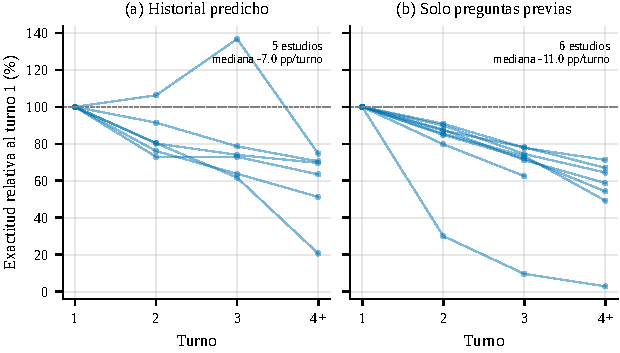
\includegraphics[width=4.14in,height=0.85\textheight,keepaspectratio]{pi5_degradacion}
\caption{Degradación de la exactitud a lo largo de los turnos (sistema propuesto, normalizada al turno 1; turnos $\geq$ 4 agrupados en «4+»), separada por el tipo de historial usado en la evaluación: (a) historial predicho; (b) solo preguntas previas. Valores por turno extraídos de las tablas de cada estudio y verificados en la página citada. Sin curvas con al menos tres turnos para: historial gold, no reportado. Los grupos de turno contienen preguntas distintas, por lo que la pendiente mezcla profundidad y dificultad; las pendientes no se agrupan entre estratos.}
\label{fig:pi5_degradacion}
\end{figure*}


El tipo de historial usado en la evaluación (\cref{tab:pi5}) es predicho en 31 estudios (43,1~\%), solo preguntas en 19 (26,4~\%), de referencia (\en{gold}) en 5 (6,9~\%) y no reportado o no extraído en 20 (27,8~\%). Un total de 38 estudios (52,8~\%) reportan degradación por turno, 10 (13,9~\%) errores de \en{join} y 7 (9,7~\%) discuten la contaminación del \en{benchmark}. En la muestra independiente de la autora, el historial coincidió en 3 de 5 estudios (60,0~\%); las discrepancias correspondieron a SUQL~\cite{Liu2024SUQL} y DIR~\cite{Li2023DIR}, y la primera se corrigió a SOLO\_PREGUNTAS. La estratificación de PI5 depende, por tanto, de una codificación verificada de forma independiente en 3 de 5 estudios de la muestra.
% fuente: PI5.md

La \cref{fig:pi5_degradacion} presenta la degradación por turno, con los estratos separados y sin agruparlos. En el estrato predicho hay 6 curvas de 5 estudios, con una pendiente mediana de $-7{,}0$~pp por turno (rango de \degPredMin{} a \degPredMax{}~pp por turno). En el estrato de solo preguntas hay 8 curvas de 6 estudios, con una mediana de $-11{,}0$~pp por turno (rango de \degSoloMin{} a \degSoloMax{}~pp por turno). Ninguna curva con al menos tres turnos corresponde al historial de referencia ni al no reportado. Todas las pendientes individuales son negativas en ambos estratos; por ejemplo, la de IGSQL~\cite{Cai2020IGSQL} en SParC es de $-16{,}95$~pp por turno (historial predicho) y la de QURG~\cite{Chai2023QURG} en SParC de $-10{,}62$~pp (solo preguntas). Los valores relativos superiores al 100~\% de la figura indican que algunos grupos de turnos posteriores puntúan más que el turno 1. Los grupos de turno contienen preguntas distintas, por lo que la pendiente mezcla la profundidad del turno con la dificultad de las preguntas, y las comparaciones entre filas son descriptivas.
% fuente: PI5.md, revision_4f.json (A9_degradacion)

\subsection{Sesgos de notificación y análisis de sensibilidad complementarios}
\label{sec:res-sesgos}
% PRISMA ítems 20d (sensibilidad) y 21 (sesgos de notificación)

Varios campos de la extracción figuran como no reportados o no extraídos en una parte amplia de los estudios del Nivel 2: la técnica de restauración del contexto en 25 de 72 (34,7~\%), el mecanismo de autocorrección en 46 de 72, el historial de la evaluación en 20 de 72 y los campos descriptivos del grafo en 64 de 72. Los contrastes con dirección negativa son escasos: se registra un estudio en la reescritura de la pregunta, uno en SQL o resultados previos y uno en la aclaración, entre otros.
% fuente: PI1.md, PI2.md, PI4.md, PI5.md

La reincorporación de los \nBajoUmbral{} estudios bajo el umbral de validez no modificó las medianas de PI1 ni de PI2. En PI3 la mediana de otros componentes pasó de \efPItresOtrosMed{} a \efPItresOtrosMedTodos{}~pp y en PI4 la de otros componentes de \efPIcuatroOtrosMed{} a \efPIcuatroOtrosMedTodos{}~pp, y la clase de autocorrección por ejecución pasó de \efAutocorrN{} a \efAutocorrNTodos{} estudios, con una mediana de \efAutocorrMedTodos{}~pp. Al excluir los preprints, la mediana de SQL o resultados previos pasó de \efSQLPrevMed{} a \efSQLPrevMedSinPre{}~pp (\efSQLPrevNSinPre{} estudios) y la de vinculación de esquemas de \efVincMed{} a \efVincMedSinPre{}~pp (\efVincNSinPre{} estudios); las demás medianas variaron poco o nada. La clase de aclaración no figura en el análisis sin preprints. Las sensibilidades de D4 se presentan en la \cref{sec:res-d4}.
% fuente: PI1.md, PI3.md, PI4.md, PI2.md

Los informes no recuperados corresponden a 148 de señal de un turno y 43 de señal multiturno. Con el supuesto extremo de que todos cuentan en el denominador y los de señal multiturno también en el numerador, D4 es de \DcuatroCotaK/\DcuatroCotaN{} (\DcuatroCotaPct~\%; IC 95~\% de \DcuatroCotaICinf{} a \DcuatroCotaICsup~\%); la estimación probabilística da D4 $\approx$ \DcuatroProbPct~\%.
% fuente: PI0.md, revision_4f.json (A7_cota_probabilistica)
%%%% END

